\documentclass{beamer}
% Nächstes Auskommentieren um jedes \pause zu 'deaktivieren'!
%\documentclass[handout]{beamer}

\usepackage{talk_BeamerColor}
\usepackage{res/meta/meta}
\usepackage[pantoneblack7,english]{talk_wwustyle_LA}

\usepackage[ngerman]{babel}
\usepackage[utf8]{inputenc}
\usepackage[T1]{fontenc}

% --- Paket um Grafiken im Dokument einbetten zu koennen
\usepackage{graphicx}
\usepackage{caption}
\usepackage{subfigure}
\usepackage{wrapfig}
\usepackage{tikz}

% --- Pakete fuer mathematischen Textsatz
\usepackage{amsmath}
\usepackage{amssymb}
\usepackage{empheq}
\usepackage{dsfont}		
\usepackage{amstext}
\usepackage{amsfonts}
\usepackage{amsthm}
\usepackage{wasysym}

% --- Paket erweitert deutlich die Verwendung von Farben aus dem Paket 'graphicx'
\usepackage{color}

% --- Paket um Quellcode sauber zu formatieren
\usepackage{listings}

% --- Darstellung von Pseudocode und mehr (algorithmicx packages)
\usepackage{algorithm}
\usepackage{algpseudocode}

%% Physikalisches
\usepackage{nicefrac}
\usepackage{units}
\usepackage{siunitx}
\sisetup{
  inter-unit-product 	=	$\cdot$,
  fraction-function   	= 	\nicefrac,
  load-configurations 	= 	abbreviations,
  per-mode            	= 	fraction,
  separate-uncertainty	=	true,
  output-decimal-marker	=	{.}
  }   
\usepackage{isotope}

%% Aufgabenverwaltung
\usepackage[textwidth=2cm,% Breite der Todo-Eintr�ge
            textsize=footnotesize,% Schriftgr��e der Eintr�ge
            english,% deutsche Beschriftungen
            shadow,% Schlagschatten f�r Boxen (weils so h�bsch ist)
            colorinlistoftodos]{todonotes}% farbige Markierungen f�r unterschiedliche Aufgabentypen
\newcommand{\detail}[1]{\todo[color=Green,inline]{detail: #1}~}% Details k�nnten hinzugef�gt werden
\newcommand{\litcheck}[1]{\todo[color=LightSteelBlue,inline]{refcheck: #1}~}% muss noch einmal �berpr�ft werden
\newcommand{\src}[1][]{\todo[color=Tomato,inline]{reference! #1}~}% Quelle fehlt

% % Zusätzliches:
\usepackage{braket}
\usepackage{epstopdf}
\usepackage{pgfpages}
\usepackage{csquotes}

\newlength{\halftextwidth}
\setlength{\halftextwidth}{\textwidth}
\divide\halftextwidth by 2

% --- Einstellungen

\author{NiMoNa 2016}
\title{Konnektivität im Gehirn}
%\institutelogo{Logo on title frame}
%\institutelogosmall{Logo on other frames}
\subtitle{Lutz Althüser, Tobias Frohoff-Hülsmann, Victor Kärcher,\\ Lukas Splitthoff, Timo Wiedemann}
\date[08.06.2016]{08. Juni, 2016}

% --- Beginn des Dokuments

\begin{document}

\begin{frame}[plain]
	  \maketitle
\end{frame}

\begin{frame}{Überblick}
	\tikz[remember picture,overlay]
		  \node at ([xshift=-2.5cm,yshift=-4.75cm]current page.north east)
		  {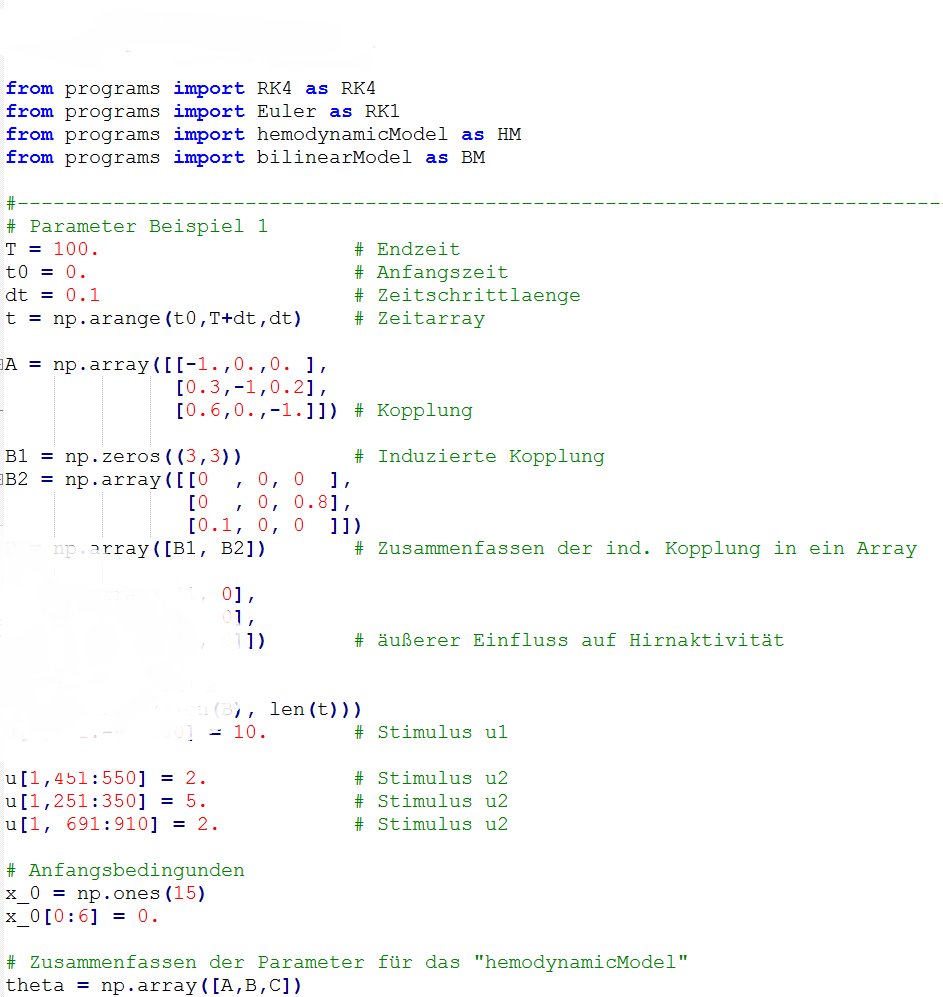
\includegraphics[height=7cm,angle=-7.5,keepaspectratio]{res/toc_2.png}};
	  \tableofcontents
\end{frame}

\section{Motivation und Ziel}
\section{Die Modelle}
\subsection{Lineares Modell}
	\begin{frame}{Einleitung in DCM}
		\begin{columns}
		\column[t]{6cm}
		\begin{figure}
			\centering
			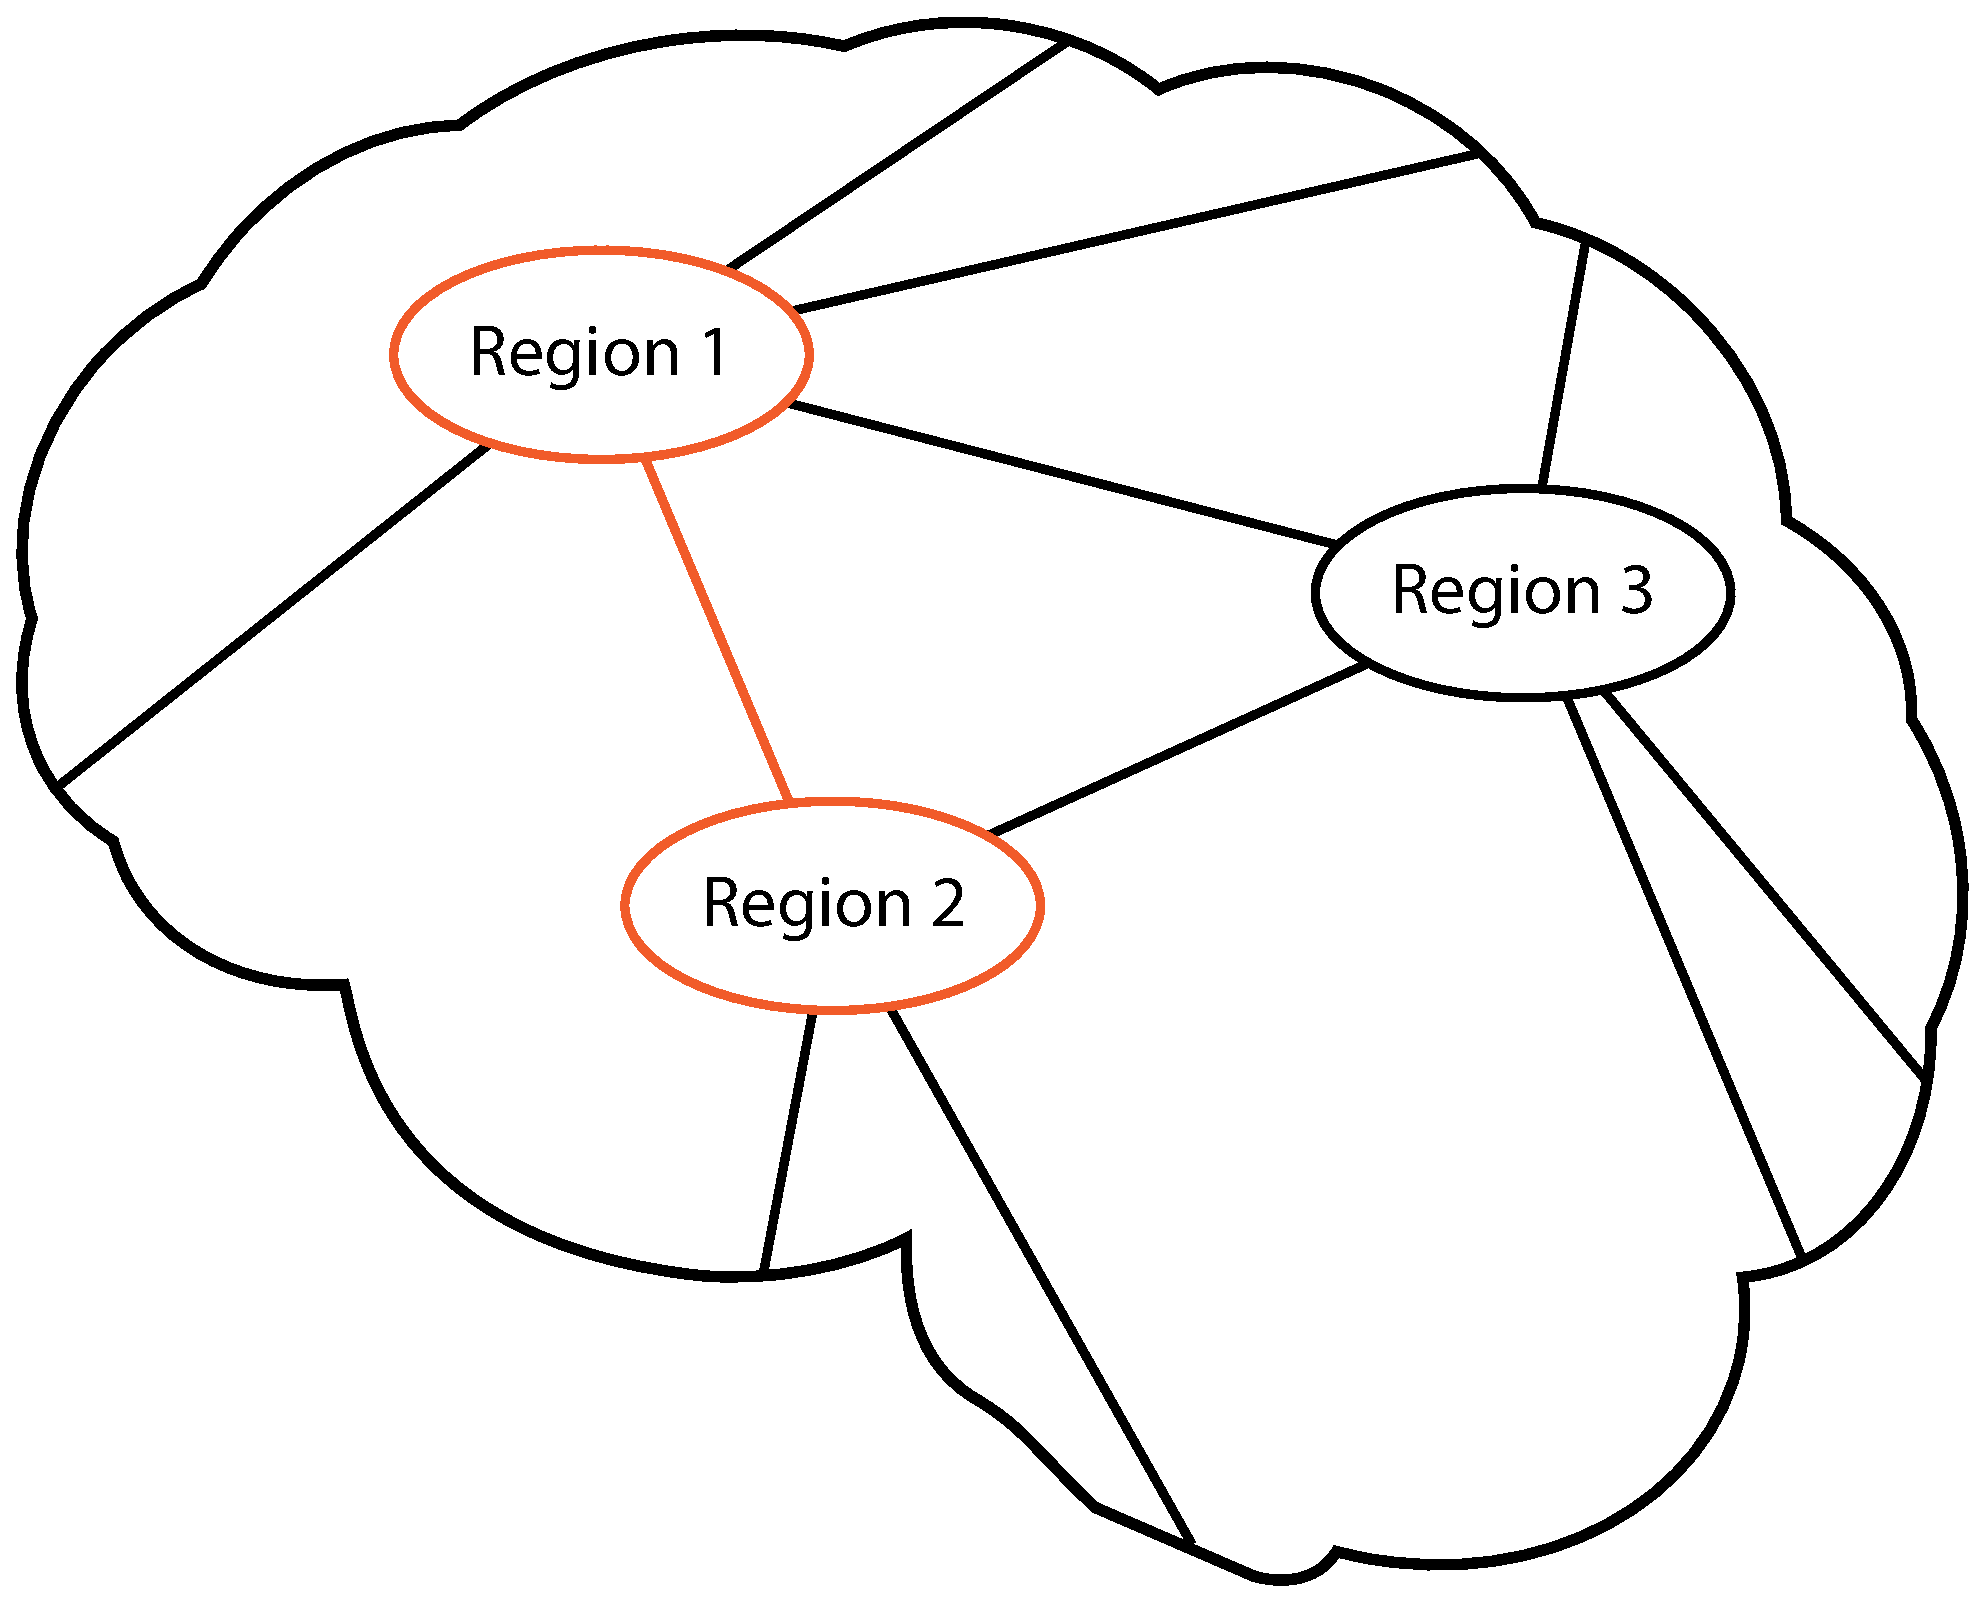
\includegraphics[width=0.85\linewidth]{res/brain_01.eps}
			\caption{Interaktion zwischen verschiedenen Hirnregionen.}
			\label{fig:brain_01}
		\end{figure}
		\column[t]{6cm}
		Konektivität im Gehirn\\
		Mathematische Modellierung von Interaktionen zwischen mehreren Regionen des Gehirns\\
		\vspace{0.5cm}
		Ziel: Austellen eines realistischen neuronalen Modells der interagierenden Gehirnregionen
		\end{columns}
	\end{frame}
	
	\begin{frame}
		Rückschlüsse auf die Verschaltung von Hirnregionen zu ziehen und zu verstehen, wie diese von Veränderungen in der neuronalen Aktivität beeinflusst wird\\
		Äquivalent der DCM ist die FMRT ...\\
		\vfill
		Messung der Veränderung vom Blutfluss - BOLD Signal
	\end{frame}
	
	\begin{frame}
		in diesem Fall ist DCM ein ...
	\end{frame}
	
\subsection{Bilineraes Modell}
	\begin{frame}{Bilineares Modell}
		Gehirn als nicht-lineares, deterministisches, dynamisches System 
		\begin{figure}[H]
			\begin{center} \label{fig: bilinearesModell}
				\includegraphics[scale=0.4]{res/bilinearesModell.eps}
				\caption{Bilineares Modell der Netzwerkgröße 3}
			\end{center}
		\end{figure}		
			
		\textbf{Annahme:}
		\begin{itemize}
			\item direkter Einfluss: Eingangssignal $ u_1 $ $ \rightarrow $ Veränderung von Zustandsvariablen (z.B. neuronaler Aktivität)
			\item indirekter Einfluss: Eingangssignal $ u_2 $ $ \rightarrow $ Veränderung der eff. Konnektivität
		\end{itemize}
			
	\end{frame}
	
	\begin{frame}{}
		\[\dot{z}=(A+\sum_{j}u_jB^j)z+Cu\]
		  \[
		 A=\left(\begin{array}{ccc} 
		  a_{11} &  a_{12} & a_{13} \\a_{21} &  a_{22} & a_{23} \\a_{31} &  a_{32} & a_{33}
		  \end{array}\right) 
		  \]
		  \[
		  B=\left(\begin{array}{ccc} 
		  b_{11} &  b_{12} & b_{13} \\b_{21} &  b_{22} & b_{23} \\b_{31} &  b_{32} & b_{33}
		  \end{array}\right) 
		  \]
		  \[
		  C=\left(\begin{array}{cc} 
		  c_{11} &  c_{12} \\c_{21} &  c_{22} \\c_{31} &  c_{32} 
		  \end{array}\right) 
		  \]
	\end{frame}
	
\subsubsection{Hämodynamisches Modell}
\begin{frame}{Vergleichbarkeit}
Bilineare Modell $\Rightarrow$ Gehirnaktivitäten $z_i(t)$\\~\\
\pause
Experiment (funktionelle MRT)$\Rightarrow$ BOLD-Signal/Kontrast $y_i(t)$\\
\hspace{3cm} $\approx$ Sauerstoffgehalt der roten Blutkörperchen 
\begin{figure}
{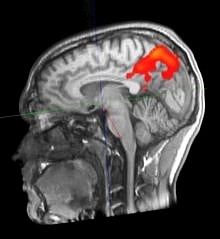
\includegraphics[width=4.4cm]{res/bold_signal.jpg}}
\end{figure}
\end{frame}

\begin{frame}{Hämodynamisches Modell}
4 biophysikalische Zustandsvariablen übermitteln $z_i(t)\rightarrow y_i(t)$:\\
$s_i(t)$: Zusammenfassung mehrerer neurogener Signale\\$ f^{in}_i(t)$: (sauerstoffreicher) Blutzufluss \\$ v_i(t)$: Venenvolumen \\$ q_i(t)$: Desoxyhämoglobinkonzentration~\\~\\
Biophysikalisch:~\\
$\dot{s}_i=z_i-\kappa s_i -\gamma (f^{in}_i-1)$\\
$\dot{f}^{in}_i=s_i$\\
$\dot{v}_i=\frac{1}{\tau}(f^{in}_i-f^{out}_i)=\frac{1}{\tau}(f^{in}_i-v_i^{1/\alpha})$\\
$\dot{q}_i=\frac{1}{\tau}(f^{in}_iE_i/\rho-v_i^{1/\alpha}q_i/v_i)$\\~\\
BOLD-Signal (fMRT):\\ $y_i=V_0(k_1(1-q_i)+k_2(1-q_i/v_i)+k_3(1-v_i))$
\end{frame}

\section{Numerische Methoden}
\subsection{Euler-Verfahren}
	\begin{frame}{Euler-Verfahren}
		explizites Verfahren
	\end{frame}
	
\subsection{Runge-Kutta-Verfahren (4. Ordnung)}
	\begin{frame}{Runge-Kutta-Verfahren (4. Ordnung)}
		Analyse der effektiven Konnektivität
	\end{frame}

\section{Theoretische Experimente}
\subsection{linear}
	\begin{frame}{Numerisches Experiment - linear}
		Analyse der effektiven Konnektivität
	\end{frame}
\subsection{bilinear}
	\begin{frame}{Numerisches Experiment - bilinear}
		Analyse der effektiven Konnektivität
	\end{frame}
\subsection{hemodynamisch}
	\begin{frame}{Numerisches Experiment - hemodynamisch}
		Analyse der effektiven Konnektivität
	\end{frame}

\section{Literatur}
	\begin{frame}{Literatur}
		\begin{itemize}
			\item \textit{Dynamic causal modelling} \\ {\small K.J. Friston et al. / NeuroImage 0 (2003)} \\ {\footnotesize \url{web.mit.edu/swg/ImagingPubs/connectivity/Dcm_Friston.pdf}}
%			\item \textit{{\small Bayesian Estimation of Dynamical Systems: An Application to fMRI}} \\ {\small K.J. Friston / NeuroImage (2002)} \\ {\footnotesize \url{www.sciencedirect.com/science/article/pii/S1053811901910444}}
		\end{itemize}
	\end{frame}



\begin{frame}
	\frametitle{Designfeatures}
	\begin{block}{Hervorhebungen}
	 \textbf{Wenn man Dinge hervorheben möchte nutzt man entweder Fettdruck,} \textit{ kursive Schrift} \alert{ oder das Schlüsselwort "alert"}. Auch "itemize"-Umgebungen werden von der Stilvorlage überschrieben:
	\end{block}
	\pause
	\begin{itemize}
	 \item So wird sichergestellt,
	 \item dass alle Elemente der Präsentation 
	 \item dieselbe Farbe nutzen.
	\end{itemize}
	\begin{alertblock}{Achtung!}
	 Hier kommt Rot ins Spiel!	
	\end{alertblock}
	\begin{exampleblock}{Beispiel}
	 Hier kommt Grün ins Spiel!
	\end{exampleblock}
\end{frame}

\end{document}
